\documentclass[11pt,a4paper]{article}
\usepackage{acl2015}
\usepackage{times}
\usepackage{latexsym}
% \setlength\titlebox{5cm}    % Expanding the titlebox

%%% Custom additions %%%
% \usepackage{hyperref}
\usepackage{url}
\usepackage[leqno, fleqn]{amsmath}
\usepackage{amssymb}
\usepackage{qtree}
\usepackage{graphicx}
\usepackage{booktabs}
\usepackage{colortbl}
% \usepackage{caption}
\usepackage{subcaption}
\usepackage{xcolor}
\usepackage{color}
\usepackage{tikz}
\usepackage{todonotes}

\newcount\colveccount
\newcommand*\colvec[1]{
        \global\colveccount#1
        \begin{bmatrix}
        \colvecnext
}
\def\colvecnext#1{
        #1
        \global\advance\colveccount-1
        \ifnum\colveccount>0
                \\
                \expandafter\colvecnext
        \else
                \end{bmatrix}
        \fi
}


\newcommand{\nateq}{\equiv}
\newcommand{\natind}{\mathbin{\#}}
%\newcommand{\natneg}{\raisebox{2px}{\tiny\thinspace$\wedge$\thinspace}}
\newcommand{\natneg}{\mathbin{^{\wedge}}}
\newcommand{\natfor}{\sqsubset}
\newcommand{\natrev}{\sqsupset}
\newcommand{\natalt}{\mathbin{|}}
\newcommand{\natcov}{\mathbin{\smallsmile}}

\newcommand{\plneg}{\mathop{\textit{not}}}
\newcommand{\pland}{\mathbin{\textit{and}}}
\newcommand{\plor}{\mathbin{\textit{or}}}

%%%%%%%%%%%%%%%%%%%%%%%%%%%%%%%%%%%%%%%%%%%%%%%%%%%%%%%%%%%%%%%%%%%%%%
%%%%% Code to simulate natbib's citealt, which prints citations with
%%%%% no parentheses:

\makeatletter
\def\citealt{\def\citename##1{{\frenchspacing##1} }\@internalcitec}
\def\@citexc[#1]#2{\if@filesw\immediate\write\@auxout{\string\citation{#2}}\fi
  \def\@citea{}\@citealt{\@for\@citeb:=#2\do
    {\@citea\def\@citea{;\penalty\@m\ }\@ifundefined
       {b@\@citeb}{{\bf ?}\@warning
       {Citation `\@citeb' on page \thepage \space undefined}}%
{\csname b@\@citeb\endcsname}}}{#1}}
\def\@internalcitec{\@ifnextchar [{\@tempswatrue\@citexc}{\@tempswafalse\@citexc[]}}
\def\@citealt#1#2{{#1\if@tempswa, #2\fi}}
\makeatother

%%%%%%%%%%%%%%%%%%%%%%%%%%%%%%%%%%%%%%%%%%%%%%%%%%%%%%%%%%%%%%%%%%%%%%


% Strikeout
\newlength{\howlong}\newcommand{\strikeout}[1]{\settowidth{\howlong}{#1}#1\unitlength0.5ex%
\begin{picture}(0,0)\put(0,1){\line(-1,0){\howlong\divide\unitlength}}\end{picture}}

\newcommand{\True}{\texttt{T}}
\newcommand{\False}{\texttt{F}}
\usepackage{stmaryrd}
\newcommand{\sem}[1]{\ensuremath{\llbracket#1\rrbracket}}

\newcommand{\mynote}[1]{{\color{blue}#1}}

\newcommand{\tbchecked}[1]{{\color{red}#1}}

\usepackage{gb4e}
\noautomath

\def\ii#1{\textit{#1}}
\newcommand{\word}[1]{\emph{#1}}

%%%%%%%%%%%%%%%%%%%%%%%%%%%%%%%%%%%%%%%%%%%%%%%%%%%%%%%%%%%%%%%%%%%%%%
%%%%% Code to simulate natbib's citealt, which prints citations with
%%%%% no parentheses:

\makeatletter
\def\citealt{\def\citename##1{{\frenchspacing##1} }\@internalcitec}
\def\@citexc[#1]#2{\if@filesw\immediate\write\@auxout{\string\citation{#2}}\fi
  \def\@citea{}\@citealt{\@for\@citeb:=#2\do
    {\@citea\def\@citea{;\penalty\@m\ }\@ifundefined
       {b@\@citeb}{{\bf ?}\@warning
       {Citation `\@citeb' on page \thepage \space undefined}}%
{\csname b@\@citeb\endcsname}}}{#1}}
\def\@internalcitec{\@ifnextchar [{\@tempswatrue\@citexc}{\@tempswafalse\@citexc[]}}
\def\@citealt#1#2{{#1\if@tempswa, #2\fi}}
\makeatother

%%%%%%%%%%%%%%%%%%%%%%%%%%%%%%%%%%%%%%%%%%%%%%%%%%%%%%%%%%%%%%%%%%%%%%


%%% %%%

\title{Tree-structured composition in neural networks without tree-structured architectures}

%\Thanks{}}

%\author{First Author \\
%  Affiliation / Address line 1 \\
%  Affiliation / Address line 2 \\
%  Affiliation / Address line 3 \\
%  {\tt email@domain} \\\And
%  Second Author \\
%  Affiliation / Address line 1 \\
%  Affiliation / Address line 2 \\
%  Affiliation / Address line 3 \\
%  {\tt email@domain} \\}

\date{}

\makeatletter
\newcommand{\@BIBLABEL}{\@emptybiblabel}
\newcommand{\@emptybiblabel}[1]{}
\definecolor{black}{rgb}{0,0,0}
\makeatother
\usepackage[breaklinks, draft, colorlinks, linkcolor=black, urlcolor=black, citecolor=black]{hyperref}

\begin{document}
\maketitle

\begin{abstract}
Tree-structured neural networks aim to deliver a robust and principled method for representing sentence meaning, but these models largely have not outperformed simpler sequence-based models by substantial margins. We hypothesize that sequence models like LSTMs are able to discover and implicitly use the same kinds of recursive compositional structures that the tree-structured ones are built around---at least in cases where there are clear cues to that structure in the data---mitigating the advantage of the tree-structured models. We investigate this possibility by evaluating both models on an artificial task for which recursive compositional structure is crucial, and find that the sequence model is able to exploit the underlying structure, though it is less efficient at learning than the tree models, only succeeding after exposure to a larger and richer set of training data.
\end{abstract}

\section{Introduction}\label{sec:introduction}

The semantic concepts of entailment and contradiction are central to
all aspects of natural language meaning
\cite{Katz72,vanBenthem08NATLOG}, from the lexicon to the content of
entire texts. Thus, \emph{natural language
  inference} (NLI) --- characterizing and using these relations in
computational systems
\cite{dagan2006pascal,MacCartney09,maccartney2009extended} --- is
essential in tasks ranging from information retrieval to semantic
parsing to commonsense reasoning.

NLI has been addressed using a wide variety of techniques, including
those grounded in syntactic structures, knowledge bases, and symbolic
logic. In recent years, it has become an important testing ground for
approaches employing \emph{distributed} word and phrase
representations. Distributed representations excel at capturing
relations based in similarity, but it is less clear that they can be
trained to support the full range of logical inferences required for
NLI. In the SemEval 2014 task aimed at evaluating distributed
representations for NLI, the best-performing systems relied heavily on
additional features and reasoning capabilities
\cite{marelli2014semeval}.

Our primary objective in this paper is to provide a new empirical
evaluation of a wide range of models for distributed semantic
representations in the context of NLI. However, in our view, the
existing corpus resources in this area do not permit such an
assessment. They are generally too small for training modern
data-intensive, wide-coverage models, and they are often beset with
indeterminacies of event and entity coreference that significantly
impact annotation quality.

To address this, we present a new corpus of sentence pairs labeled for
entailment, contradiction, and semantic independence. At 550,152
sentence-pairs, this corpus is orders of magnitude larger than all
other resources of its type. And, in contrast to many such resources,
all of the sentences were written by humans in a grounded,
naturalistic context. In a separate validation phase, we collected
four additional judgments for each label for 56,941 of the examples,
and 98\% of cases emerge with a gold label, which attests to the high
quality of the data.

In this paper, we use this corpus to evaluate a wide variety of models
for natural language inference, including rule-based systems, simple
linear classifiers, and compositional neural networks. We find that
Tree-Structured Long Short-Term Memory networks (TreeLSTMs;
\citealt{tai2015improved,le2015compositional}) achieve the best
performance. In addition, we enhance the case for TreeLSTMs by showing
that its representations, trained on our corpus, perform well in a
disparate set of additional semantic tasks.  The success of these
transfer-learning experiments is also a testament to the centrality
of NLI in semantics.


%%%%%%%%%%%%%%%%%%%%%%%%%%%%%%%%%%%%%%%%%%%%%%%%%%%%%%%%%%%%%%%%%%%%%%


% One point of comparison that might be good to set up (maybe not in these words, this is Sam's sketch):

% Translation can also be used to train/evaluate NNs, and also demands some degree of sensitivity to compositional syntactic and semantic structure. Plus, it's easier to get good data for that task. But NLI is the better benchmark for developing NNs for language understanding, because:

% (i) Typical translation tasks require natural language generation, which is a separate difficult problem that must be learned in parallel with the semantic encoding task of interest, making results harder to interpret. We can just a vanilla well-understood classifier on top of our sentence model.

% (ii) Contradiction vs. entailment decisions in particular specifically target the abilities of NN models to learn lexical and phrasal representations (like alternation) that don't resemble similarity, either in their correlation with distributional information or their transitivity behavior. MT doesn't seem to have a good parallel to this. Since modeling similarity is almost the only aspect of NN behavior in NLP that's reasonably well understood and basically known to work, using a benchmark that explicitly demands something more sophisticated than this is likely to pay off by better exposing the weaknesses of current standard models.

% It might be also worth making an explicit comparison with sentiment as a benchmark, but that's low-hanging fruit.
\section{Recursive structure}\label{sec:recursion}

% TODO: Check on citation for clark/coecke/sadr 2011

% Run baseline anyway?

% TODO: Clean up next sent.
Recursive compositional structure is a prominent feature of natural language. 
This section examines the 
question of whether our models are able to learn a 
compositional semantics over such recursive structures.
In our evaluations, we exploit the fact that our logical language
is infinite by testing on strings that are longer and more complex
than any seen in training.

% Consider, for example, \ii{Alice said hello}, \ii{Bob said that Alice
%   said hello}, and \ii{Carl thinks that Bob said that Alice said
%   hello}. Overt recursion of this kind is easy to find, and
% theoretical accounts of natural language syntax and semantics rely
% heavily on recursive structures. In order for a model to be able to
% accurately learn natural language meanings, then, we expect that it
% would need to be able to learn to represent the meanings of function
% words in a such a way that they are able to behave correctly when
% taking their own outputs as input. In evaluating the model, we take
% advantage of the fact that recursive structures of this kind define
% potentially infinite languages by testing the model on strings that
% are longer and more complex than any seen in testing.

\paragraph{Experiments}
As in \S\ref{sec:join}, we test this phenomenon within the
framework of natural logic, but we now replace the unanalyzed symbols
from that experiment with complex formulae. These formulae
represent a truth-functionally complete classical propositional logic:
each atomic symbol is a variable over the domain \{$\True$, $\False$\}, and the only
operators are truth-functional ones.  Table~\ref{tab:pl} defines this
logic, and Table~\ref{tab:plexs} gives some examples of relational
statements that we can make in these terms. To compute these relations
between statements, we exhaustively enumerate the sets of assignments
of truth values to propositional variables that would satisfy each of
the statements, and then we convert the set-theoretic relation between
those assignments into one of the seven relations in
Table~\ref{b-table}. As a result, each relational statement represents
a valid theorem of the propositional logic.

\begin{table}[tp]
  \centering\small
  \begin{subtable}[t]{0.45\textwidth}
    \centering
    \begin{tabular}[t]{l l}
      \toprule
      Formula     & Interpretation \\
      \midrule
      $p_1$, $p_2$, $p_3$, $p_4$, $p_5$, $p_6$ & $\sem{x} \in \{\True, \False\}$ \\
      $\plneg \varphi$ & $\True$ iff $\sem{\varphi} = \False$ \\
      $(\varphi \pland \psi)$ & $\True$ iff $\False \notin \{\sem{\varphi}, \sem{\psi}\}$ \\
      $(\varphi \plor \psi)$  & $\True$ iff $\True \in \{\sem{\varphi}, \sem{\psi}\}$ \\
      \bottomrule
    \end{tabular}    
    \caption{Well-formed formulae. $\varphi$ and $\psi$
      range over all well-formed formulae, and $\sem{\cdot}$ is
      the interpretation function mapping formulae into $\{\True,
      \False\}$.}\label{tab:pl}
  \end{subtable}
  \begin{subtable}[t]{0.45\textwidth}
    \centering\vspace{4mm}
    \begin{tabular}[t]{r c l}
      \toprule
      $\plneg p_3$        & $\natneg$ & $p_3$ \\
      $\plneg \plneg p_6$ & $\nateq$  & $p_6$ \\
      $p_3$               & $\natfor$ & $(p_3 \plor p_2)$ \\
      $(p_1 \plor (p_2 \plor p_4))$               & $\natrev$ & $(p_2 \pland  \plneg p_4)$ \\
      %$(a \natfor b)$   & $\nateq$  & $(b \natrev a)$ \\	
      $\plneg\, (\plneg p_1 \pland \plneg p_2)$ & $\nateq$ & $(p_1 \plor p_2)$ \\ 
      \bottomrule
    \end{tabular}
    \caption{Examples of the type of statements used for training and testing. These are relations between
      well-formed formulae, computed in terms of sets of satisfying
      interpretation functions $\sem{\cdot}$.}\label{tab:plexs}
  \end{subtable}
  \caption{Natural logic relations over sentences of propositional logic.}  
  \label{prop-figure}
\end{table}

Socher et al.~\shortcite{socher2012semantic} show that a matrix-vector RNN
model somewhat similar to our RNTN can learn boolean logic, 
a logic where the atomic symbols are simply the
values $\True$ and $\False$. While learning the operators of that logic is not trivial, the outputs of
each operator can be represented accurately by a single bit.
In the more demanding task presented here, the atomic symbols are variables over these values, and the sentence vectors must thus be able to distinguish up to $2^{64}$ distinct conditions on valuations. Relational expressions between these conditions are essentially theorems of propositional logic, and to succeed, the model must learn to approximate the behavior of a theorem prover.
% TODO: Condense this para, and move bulk to footnote.

In our experiments, we randomly generate unique pairs 
of formulae and compute the relation that holds for each pair.
We discard pairs in which either statement is either a tautology or a
contradiction, for which the seven relations in
Table~\ref{b-table} are undefined. The resulting set of formula pairs is
then partitioned into 13 bins according the number of logical operators in
the longer of the two formulae. We then sample 20\% of each
bin for a held-out test set.

If we do not implement any constraint that the two statements being
compared are similar in any way, then the generated data are dominated
by statements in which the two formulae refer to largely separate
subsets of the six variables, which means that the $\natind$ relation
is almost always correct.  In an effort to balance the distribution of
relation labels without departing from the basic task of modeling
propositional logic, we disallow individual pairs of statements from
referring to more than four of the six propositional variables.

In order to test the model's generalization to unseen structures, we discard
training examples with more than 4 connectives, yielding 60k short training examples,
and 21k test examples containing up to 12 connectives.
We evaluated both the RNN and RNTN\footnote{We did not run any strictly simpler baselines for this experiment because it is demonstrably impossible to perform substantially above chance on longer expressions without word order information.} on the resulting data, initializing the model parameters randomly,
including the vector representations of the six variables.


\begin{figure*}[t]
  \centering
  
\includegraphics[width=5.75in]{decayfig.eps}
%  \includegraphics[width=5.3in]{recursion\string_pairwise.eps}
  \caption{Model performance on propositional logic, by expression size.}
%    The dashed line indicates that only expressions of size four or less appeared in the training data. \textbf{Bottom:} Semantically distinct formulae should have different
%    representations. As measured by Euclidean distance, only the RNTN
%    achieves this for formulae containing more than a small number of
%    connectives (\ii{and} in this example). The RNN quickly collapses the representations,
%    failing to capture the meaning contrasts.
    
  \label{prop-results} 
  
\end{figure*}


\paragraph{Results} Figure~\ref{prop-results} shows the relationship
between test accuracy and statement length. We found that both 
models were able to perform well on unseen small test examples, 
with RNN accuracy above
98\% and RNTN accuracy above 99\% on formulae below length five.
Starting at size four, performance gradually falls with increasing
size. Training accuracy was 99.4\% for the RNN and 99.8\% for the RNTN.

The performance of these models on small unseen test examples
indicates that they learned correct approximations of the underlying
logic. These approximations are accurate enough to yield
correct answers when the composition layer is only applied a small
number of times, but that the error in the approximation grows with
increasing expression size, resulting in gradually dropping performance. 
Though imperfect, model performance on the long examples is striking. 
The RNTN classifies true examples of every class but $\nateq$ 
(which occurs only once) correctly the majority of the time, where a 
typical statement might be $( ( p_1  \pland ( p_2 \plor ( \plneg p_4 ) ) ) \plor p_3 ) \natcov ( \plneg ( ( \plneg ( ( \plneg ( p_4 \plor p_3 ) )  \plor ( ( \plneg p_3 ) \plor ( \plneg p_3 ) ) ) ) \pland ( \plneg ( ( \plneg ( ( \plneg p_3 ) \plor ( \plneg p_4 ) ) ) \plor ( \plneg p_2 ) ) ) ) )$.
% TODO: Better present examples.

It appears that the RNTN model overfit somewhat relative to the plain RNN,
performing better on the training data and short examples, but worse on longer
examples. Two factors are likely involved in this: even with the lower dimension,
the RNTN composition function has about eight times as many parameters as the
RNN, and thus more capacity to find a solution involving a large number of narrow 
generalizations that work on the training data but don't generalize well. In addition,
the RNTN used here has slightly weaker L2 regularization than the 
RNN ($\lambda_{\textit{RNN}} = 0.001$, $\lambda_{\textit{RNTN}} = 0.0003$). This
yielded better average performance, but may have facilitated this effect.


% \mynote{In an effort to better understand why model performance decays, 
%we evaluated both models on pairs of long formulae involving
%binary connectives, to assess how well they distinguish representations for semantically distinct
%formulae. We found that only the RNTN is able to learn
%substantially different representations for pairs of differing formulae like $(a \pland (a \pland a))$
% and $(a \pland (a \pland b))$ when the difference between the two is placed under multiple operators.
%The RNN separates the bare symbols by a euclidean distance of 3.5, but this falls to less than one once the two are placed under three operators, and quickly approaches zero as depth increases.
% The RNTN separates the bare symbols by 2.5, and this falls off much more gradually to 1.3 with twelve operators.}

% we discovered that this model looses information about in longer
% statements in a particularly problematic way. It appears that that
% model is unable to distinguish between two sentences when the only
% difference between those sentences is embedded within a very deep
% structure. We evaluated both models on sentences that differed in only
% one term, but for which that one term was embedded under a large
% number of conjunctions, such as the pair \ii{a (and a)} and \ii{a (and
%   b)}, or the pair \ii{a (and (a (and a)))} and \ii{a (and (a (and
%   b)))}. We then measured the Euclidean distance between the vector
% representations of the two sentences in each pair. Our findings are
% shown in Figure~\ref{prop-falloff}, and show that while the RNTN can
% distinguish the two sentences well at every size that we test, the RNN
% fails after a depth of approximately six.



\section{Testing sentence models on entailment} \label{methods}

We use the architecture depicted in Figure~\ref{fig:model:top}, which builds on the one used in \newcite{Bowman:Potts:Manning:2014}. The model architecture uses two copies of a single sentence model (a tree or sequence model) to encode the premise and hypothesis (left and right side) expressions, and then uses those encodings as the features for a multilayer classifier which predicts one of the seven relations. Since the encodings are computed separately, the sentence models must encode complete representations of the meanings of the two sentences for the downstream model to be able to succeed.

\begin{figure*}[t]
  \centering
  \begin{subfigure}[t]{0.45\textwidth}
\centering
\scalebox{0.75}{
 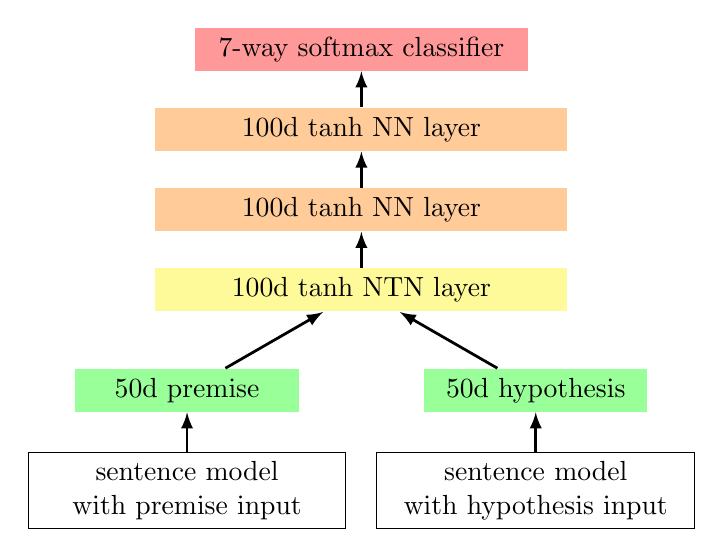
\begin{tikzpicture}
    \def\dx{21pt}
    \def\dy{29pt}

    \tikzstyle{label}=[text width=40mm,align=center]    
    \tikzstyle{softmax}=[fill=red!40,text width=40mm,align=center]
    \tikzstyle{preclass}=[fill=orange!40,text width=50mm,align=center]
    \tikzstyle{e}=[fill=green!40,text width=26mm,align=center]
    \tikzstyle{m}=[draw=black,text width=38mm,align=center]    
    
    \node[softmax]  (softmax) at (0*\dx,6*\dy) {7-way softmax classifier};
    \node[preclass]  (pc3) at (0*\dx,5*\dy) {100d $\tanh$ NN layer};
    \node[preclass]  (pc2) at (0*\dx,4*\dy) {100d $\tanh$ NN layer};
    \node[preclass,fill=yellow!40]  (pc1) at (0*\dx,3*\dy) {100d $\tanh$ NTN layer};
    \node[e]  (pe) at (-3*\dx,1.75*\dy) {50d premise};
    \node[e]  (he) at (3*\dx,1.75*\dy) {50d hypothesis};
    \node[m]  (pem) at (-3*\dx,0.5*\dy) {sentence model\\ with premise input};
    \node[m]  (hem) at (3*\dx,0.5*\dy) {sentence model\\ with hypothesis input};    
    
    \pgfsetarrowsend{latex}
    \tikzstyle{fwd} = [draw=black, line width=1pt]

          \draw [fwd] (pc3) -- (softmax);
          \draw [fwd] (pc2) -- (pc3);
          \draw [fwd] (pc1) -- (pc2);
          \draw [fwd] (pe) -- (pc1);
          \draw [fwd] (he) -- (pc1);
          \draw [fwd] (hem) -- (he);
          \draw [fwd] (pem) -- (pe);

  \end{tikzpicture}}
  
 \caption{The general architecture shared across models.}\label{fig:model:top}
  
\end{subfigure}

\begin{subfigure}[t]{0.45\textwidth}
  \centering
\scalebox{0.75}{
 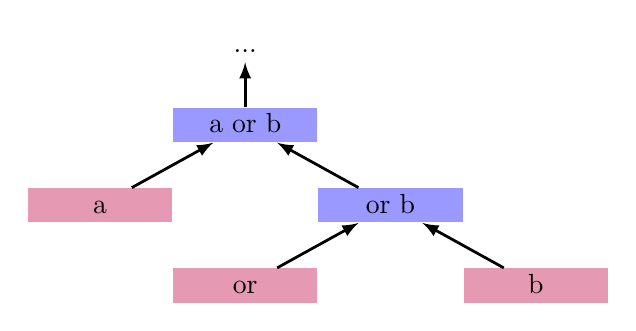
\begin{tikzpicture}
    \def\dx{21pt}
    \def\dy{29pt}


    \tikzstyle{word}=[fill=purple!40,text width=16mm,text height=2mm,align=center]
    \tikzstyle{node}=[fill=blue!40,text width=16mm,text height=2mm,align=center]
    \tikzstyle{empty}=[fill=blue!0,text width=8mm,text height=2mm,align=center]

    \node[empty]  (null) at (0*\dx,7*\dy) {...};
    \node[node]  (aorb) at (0*\dx,6*\dy) {a or b};
    \node[word]  (a) at (-2.5*\dx,5*\dy) {a};
    \node[node]  (orb) at (2.5*\dx,5*\dy) {or b};
    \node[word]  (or) at (0*\dx,4*\dy) {or};
    \node[word]  (b) at (5*\dx,4*\dy) {b};
    
    
    \pgfsetarrowsend{latex}
    \tikzstyle{fwd} = [draw=black, line width=1pt]

          \draw [fwd] (or) -- (orb);
          \draw [fwd] (b) -- (orb);
          \draw [fwd] (a) -- (aorb);
          \draw [fwd] (orb) -- (aorb);
          \draw [fwd] (aorb) -- (null);
  \end{tikzpicture}}
  
     \caption{The architecture for the TreeRNN and TreeRNTN sentence models. Terminal nodes are learned embeddings and nonterminal nodes are either NN or NTN layers with $\tanh$ nonlinearities.}\label{fig:model:tree}
  
  \end{subfigure}
 \vspace{0.5cm}
  
\begin{subfigure}[t]{0.45\textwidth}
  \centering
\scalebox{0.75}{
 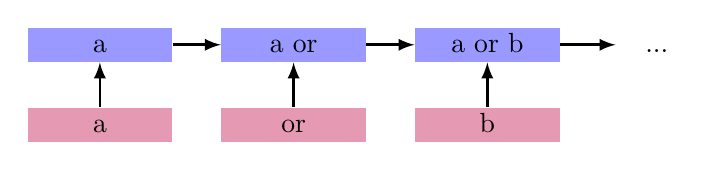
\begin{tikzpicture}
    \def\dx{35pt}
    \def\dy{29pt}


    \tikzstyle{word}=[fill=purple!40,text width=16mm,text height=2mm,align=center]
    \tikzstyle{node}=[fill=blue!40,text width=16mm,text height=2mm,align=center]
    \tikzstyle{empty}=[fill=blue!0,text width=8mm,text height=2mm,align=center]

    \node[word]  (a) at (-3*\dx,1*\dy) {a};
    \node[node]  (aN) at (-3*\dx,2*\dy) {a};
    
    \node[word]  (or) at (-1*\dx,1*\dy) {or};
    \node[node]  (orN) at (-1*\dx,2*\dy) {a or};
    
    \node[word]  (b) at (1*\dx,1*\dy) {b};
    \node[node]  (bN) at (1*\dx,2*\dy) {a or b}; 
    
    \node[empty]  (nullN) at (2.75*\dx,2*\dy) {...}; 
    
    \pgfsetarrowsend{latex}
    \tikzstyle{fwd} = [draw=black, line width=1pt]

          \draw [fwd] (or) -- (orN);
          \draw [fwd] (b) -- (bN);
          \draw [fwd] (a) -- (aN);
          \draw [fwd] (aN) -- (orN);
          \draw [fwd] (orN) -- (bN);
          \draw [fwd] (bN) -- (nullN);
          
  \end{tikzpicture}}
  
   \caption{The architecture for the LSTM sentence model. Nodes in the lower row are learned embeddings and nodes on the upper row are LSTM units.}\label{fig:model:seq}
  
    \end{subfigure}
  \caption{In our model, two copies of a sentence model---based on either tree (b) or sequence (c) models---encode the two input sentences. A multilayer classifier component (a) then uses the resulting vectors to predict a label that reflects the logical relationship between the two sentences.}
  \label{sample-figure}
\end{figure*}


\paragraph{Classifier}
The classifier component of the model consists of a combining layer which takes the two sentence representations as inputs, followed by two neural network layers, then a softmax classifier.
For the combining layer, we use a neural tensor network (NTN, \cite{chen2013learning}) layer, which sums the output of a plain recursive/recurrent neural network layer with a vector computed using two multiplications with a learned (full rank) third-order tensor parameter:
\begin{gather} 
\label{TreeRNN}
\vec{y}_{\textit{NN}} = \tanh(\mathbf{M} \colvec{2}{\vec{x}^{(l)}}{\vec{x}^{(r)}} + \vec{b}\,) \\
\label{TreeRNTN} 
\vec{y}_{\textit{NTN}} = \vec{y}_{\textit{NN}} + \tanh(\vec{x}^{(l)T} \mathbf{T}^{[1 \ldots n]} \vec{x}^{(r)})
\end{gather} 

Our model is largely identical to the model from \newcite{Bowman:Potts:Manning:2014}, but adds the two additional $\tanh$ NN layers, which we found help performance across the board, and also uses the NTN combination layer when evaluating all four models, rather than just the TreeRNTN model, so as to ensure that the sentence models are compared in as similar a setting as possible.

We only study models that encode entire sentences in fixed length vectors, and we set aside models with attention \cite{bahdanau2014neural}, a technique which gives the downstream model (here, the classifier) the potential to access each input token individually through a soft content addressing system. While attention simplifies the problem of learning complex correspondences between input and output, there is no apparent reason to believe that it should improve or harm a model's ability to track structural information like a given token's position in a tree. As such, we expect our results to reflect the same basic behaviors that would be seen in attention-based models.

\paragraph{Sentence models}
The sentence encoding component of the model transforms the (learned) embeddings of the input words for each sentence into a single vector representing that sentence. We experiment with tree-structured models (Figure~\ref{fig:model:tree}) with TreeRNN (eqn.~\ref{TreeRNN}), TreeRNTN (eqn.~\ref{TreeRNTN}), and TreeLSTM \cite{tai2015improved} activation functions. In addition, we use a sequence model (Figure~\ref{fig:model:seq}) with an LSTM activation function \cite{hochreiter1997long} implemented as in \newcite{zaremba2015recurrent}. In experiments with a simpler non-LSTM RNN sequence model, the model tended to badly underfit the training data, and those results are not included here.

\paragraph{Training} We randomly initialize all embeddings and layer parameters, and train them using minibatch stochastic gradient descent with AdaDelta \cite{zeiler2012adadelta} learning rates. Our objective is the standard negative log likelihood classification objective with L2 regularization (tuned on a separate train/test split). All models were trained for 100 epochs, after which all had largely converged without significantly declining from their peak performances.

\section{General discussion}\label{sec:discussion}

This paper evaluated two recursive models on a series of three increasingly
challenging interpretive tasks involving natural language inference:
the core labelal algebra of natural logic with entailment and
exclusion; recursive propositional logic structures; and statements
involving quantification and negation. The results suggest that RNTNs,
but not plain RNNs, have the capacity to meet the challenges of these
tasks with reasonably-sized training sets. These positive results are
promising for the future of learned representation models in the
applied modeling of compositional semantics.

Of course, challenges remain. In terms of our experimental data, even
the RNTN falls short of perfection in our more complex tasks, with
performance falling off steadily as the depth of recursion grows. It
remains to be seen whether these deficiencies can be overcome with
improvements to the model, the optimization procedures, or the
linguistic representations
\cite{sochergrounded,kalchbrenner2014convolutional}. In addition,
there remain subtle questions about how to fairly assess whether these
models have truly generalized in the way we want them to. There is a
constant tension between showing the models training data that gives
them a chance to learn the target logical functions and revealing the
answer to them in a way that leads to overfitting. The underlying
logical theories provide only limited guidance on this point.
%
%, and the fact that there is a finite universe of possible
%  expressions makes his an unavoidable issue. 
%
%  CP: I don't understand the above. It is false if taken literally;
%  our PL generates an infinte number of formulae.
%
Finally, we have only scratched the surface of the logical complexity
of natural language; in future experiments, we hope to test sentences
with embedded quantifiers, multiple interacting quantifiers, relative
clauses, and other kinds of recursive structure. Nonetheless, the
rapid progress the field has made with these models in recent years
provides ample reason to be optimistic that they can be trained to
meet the challenges of natural language semantics.

% These experiments represent one of the first attempts to reproduce any large fragment of the behavior of a complex logic within a neural network model, and the first attempt that we are aware of to address either the encoding of lexical labels or the learning of recursive operators. This presents considerable challenges in evaluating the particular models that we choose, since we cannot rely on prior results to establish that any particular amount or type of training data is sufficient to teach any model the structure of the logic. The positive results that we have found, however, are extremely promising for the future of learned representation models in the applied modeling of meaning. We have seen that recursive neural tensor networks are able to encode lexical labels accurately and encode recursive operators. We have also seen that both RNNs and RNTNs are able to handle the meanings of quantifiers in an inference setting in at least some cases. 

% There is ample room to build on these results. In the interest of fully mirroring the capacity of existing natural logics in learned models, it would be valuable to extend these experiments to cover other ways in which meanings are encoded in natural language, including challenges such as reasoning over sentences with transitive verbs or relative clauses. In addition, it would be highly informative to compare these results on standard recursive neural networks with other proposed learned models for sentence meaning, such as dependency tree RNNs \cite{sochergrounded}, Belief Propagation RNNs (TODO: cite), or convolutional RNNs \cite{kalchbrenner2014convolutional}.



%\subsubsection*{Acknowledgments}

% We thank Jeffrey Pennington, Richard Socher, and audiences at CSLI, Nuance, and BayLearn, as well as Neha Nayak for developing the SICK collapsing technique.

\bibliographystyle{acl}
\bibliography{MLSemantics} 

\end{document}
